\documentclass{article}

%Headers
\usepackage[dvips]{graphicx}    %package that does pdfs
\usepackage{color}              %this needs to be here also

\title{CS440: The Maze is on Fire}
\author{Andy Rivera, John Juarez}
\date{February 19, 2021}

\begin{document}
\maketitle

\section{Maze Generation and Project Setup}
   To generate a maze we used the function \textbf{generateMaze(int dim,double p)} it takes in the parameters of  \textit{dim} to construct a dimxdim 2D array and \textit{p} to determine the probability of a block being filled(1) or not(0).
   
   To set up the project for the path finding algorithms we created an object \textbf{Point} with the following attributes:
   \begin{itemize}
   \item Point parent (Previous location of agent)
   \item X and Y to keep track of location of agent
   \item stepsTaken (Amount of steps taken to get to the current location.)
   \item Hueristics (Estimate for A* algorithm)
   \end{itemize}

\begin{figure}[hbt!]

\centering
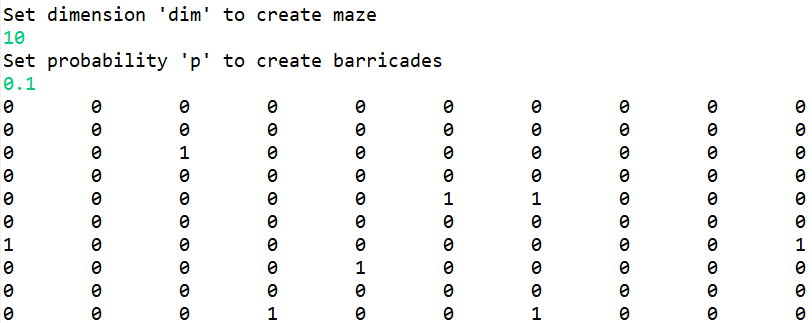
\includegraphics[width=3.5in]{maze1}\hfill
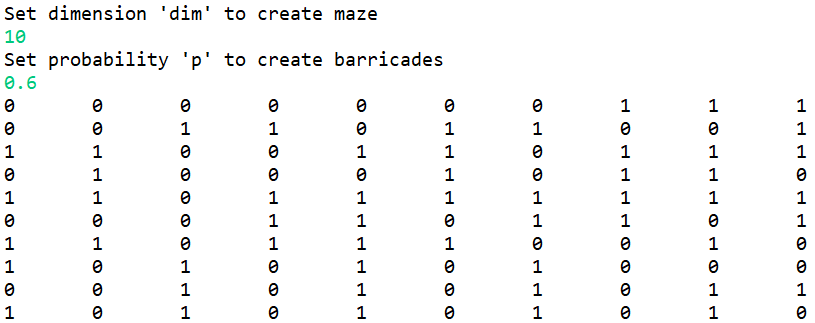
\includegraphics[width=3.5in]{maze3}

\caption{Maps generated with p = 0.1 and 0.6 respectively}
\label{fig:figure1}

\end{figure}


\section{DFS Algorithm}
  We created the method \textbf{mazeDFS(int[][] maze, Point start, Point goal).} It takes in 2 points and returns a boolean, True if there exists a path and false if no path exists between the starting point and the goal point. 
	
	With two arbituary points in the maze, DFS would be a better option because we are just determining if there is a path between the two points and not necessarily the shortest path and saving space in memory since it adds less points into the fringe.
	\begin{figure}[hbt!]

\centering
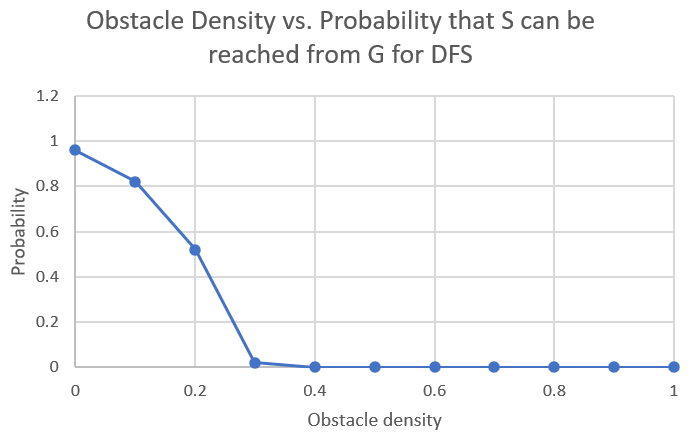
\includegraphics[width=3.5in]{DFS Plot}

\caption{obstacle density p vs probability that S can be reached from G}
\label{fig:figure2}

\end{figure}

\section{BFS and A* Algorithms}
   For our BFS algorithm, we created the method \textbf{mazeBFS(int[][] maze).} It returns the ArrayList of the points that make up the shortest path.
   
   For our A* algorithm, we created the method \textbf{mazeAStar(int[][] maze).} It uses a priority queue that prioritizes points based on an estimation that is determined by adding up the euclidean distance + the de-prioritization of steps that take you further from goal.
   \begin{figure}[hbt!]
   \centering
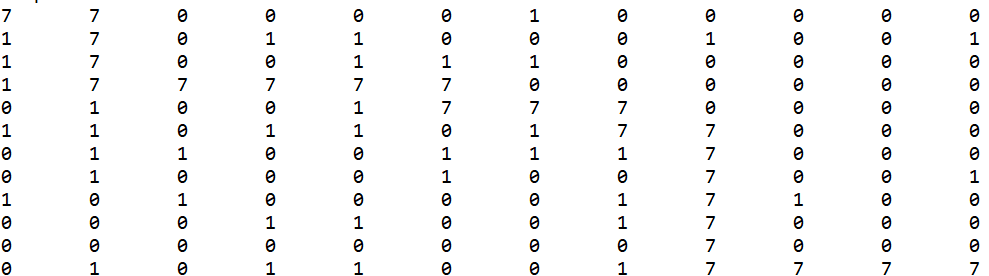
\includegraphics[width=3.5in]{BFS}

\caption{BFS Shortest path represented by 7 dim = 12 p = 0.3}
\label{fig:figure1}

\end{figure}

 \begin{figure}[hbt!]
   \centering
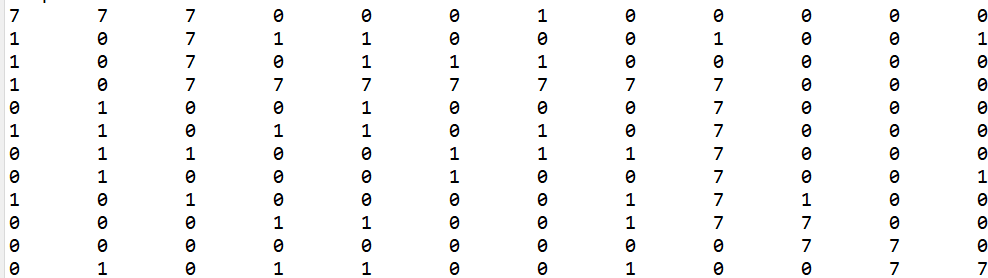
\includegraphics[width=3.5in]{astar}

\caption{A* Shortest path represented by 7 dim = 12 p = 0.3}
\label{fig:figure1}

\end{figure}
   

\section{Algorithms in less than 1 minute}	

\section{Maze is on Fire: Strategy 3}

\section{Strategies Success Rates}

\section{What if we had unlimited computational resources?}

\section{10 Seconds}





	
\end{document}